\documentclass[12pt,a4paper]{article}

% packages
\usepackage[utf8]{inputenc}
\usepackage[margin=1in]{geometry}
\usepackage{graphicx}
\usepackage{amsmath}
\usepackage{hyperref}
\usepackage{subcaption}
\usepackage{multirow}

\usepackage{listings}
\usepackage{xcolor}

% Define custom colors
\definecolor{codegreen}{rgb}{0,0.6,0}
\definecolor{codegray}{rgb}{0.5,0.5,0.5}
\definecolor{codepurple}{rgb}{0.58,0,0.82}
\definecolor{backcolour}{rgb}{0.95,0.95,0.92}

\lstdefinestyle{Rstyle}{
    language=R,
    backgroundcolor=\color{backcolour},   
    commentstyle=\color{codegreen},
    keywordstyle=\color{blue}\bfseries,
    numberstyle=\tiny\color{codegray},
    stringstyle=\color{codepurple},
    basicstyle=\ttfamily\footnotesize,
    breakatwhitespace=false,         
    breaklines=true,                 
    captionpos=b,                    
    keepspaces=true,                 
    numbers=left,                    
    numbersep=5pt,                  
    showspaces=false,                
    showstringspaces=false,
    showtabs=false,                  
    tabsize=2,
    frame=single,
    rulecolor=\color{codegray},
    morekeywords={brm, mutate, filter, rename, scale, prior, normal, exponential, lkj, trials, binomial, logit}
}

\lstset{style=Rstyle}

\usepackage{titlesec}
\newcommand{\sectionbreak}{\clearpage}

\usepackage[style=ieee]{biblatex}
\addbibresource{references.bib}

% document information
\title{Modeling Airplane Fatality Rates}
\date{}

\author{Markus Kruth \& Andreas Bogossian}


\begin{document}



\maketitle

\begin{abstract}
  This project models the fatality rates or airplane crashes from the years 1975 to 2024. For the models, we use non-hierarchical and hierarchical models with the airplane manufacturer as the hierarchy. In our project, we use two non-hierarchical and one hierarchical model to model the fatality rates of the crashes, and then compare the performance of these models. We use one non-hierarchical model with complete pooling and one with no pooling. The hierarchical model uses partial pooling, where we assume some manufacturer specific effect.
\end{abstract}

\tableofcontents


\section{Introduction}
\subsection{Motivation}
Aviation has undergone massive developments since the first commercial flight in 1914. Airplane safety has always been the top priority for airlines; a single airplane crash will drive away customers to safer perceived airlines and, of course, cost lives. Although this priority of making airplanes as safe as possible has significantly reduced the number of crashes over the years, accidents still continue to occur.

Not all accidents are the same; survivability in crashes varies significantly. Understanding which factors influence survivability in crashes remains crucial for manufacturers and airlines seeking to minimize the loss of life. While accident prevention remains the most important priority, understanding the fatality patterns when accidents do occur is equally important in discussions of airplane safety.

\subsection{Problem}
When aviation accidents occur, the fatality rates vary significantly from incidents where all passengers survive to catastrophic losses of all who were on board. This variation raises critical questions: Has the likelihood of surviving an ariplane crash improved over time? Do certain airplane manufacturers demonstrate conistently higher crash survival rates than others? How much of the variation in crash fatality rates can be attributed to crash specific details of individual accidents versus inherent airplane characteristics? These are questions that we hope to answer in our report.

\subsection{Main modeling idea}
We address these questions using hierarchical and non-hierarchical Bayesian modeling of fatality rates across aviation accidents from 1975 to 2024. In this approach we will assume that the aircrafts from the same manufacturers share some of the same characteristics, like similar design choices, engineering approaches, and safety systems. We still keep the information that all the aircrafts are similar with each other by having the high-level pooling for all the aircrafts. We will compare a partial pooling model with two different models: a complete pooling and a no pooling model.


\subsection{Data}

The dataset was obtained form a Kaggle repository created by Jonathan Ogwumike \cite{jogwums2023aircrashes}. According to the reporitory description, the dataset has been used to teach students about power BI and python.

The dataset has two notable projects linked to it. Both of the projects are written with python and either of the projects use hierarchical models to analyse the fatality rate trend. Both repositories have some sort of explaratory analysis about the data, but this is written in Python so we had to write our own analysis code again in R.

\begin{figure}[htbp]
  \centering
  \begin{subfigure}[b]{0.48\textwidth}
    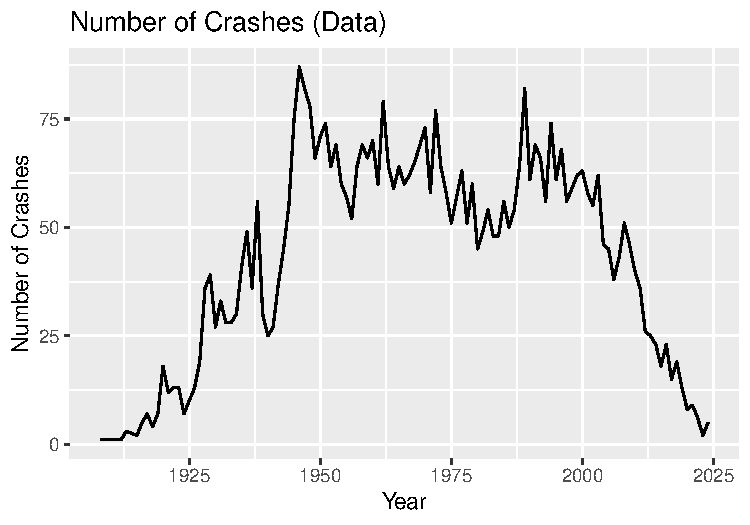
\includegraphics[width=\textwidth]{figures/crashes-data.pdf}
  \end{subfigure}
  \hfill
  \begin{subfigure}[b]{0.48\textwidth}
    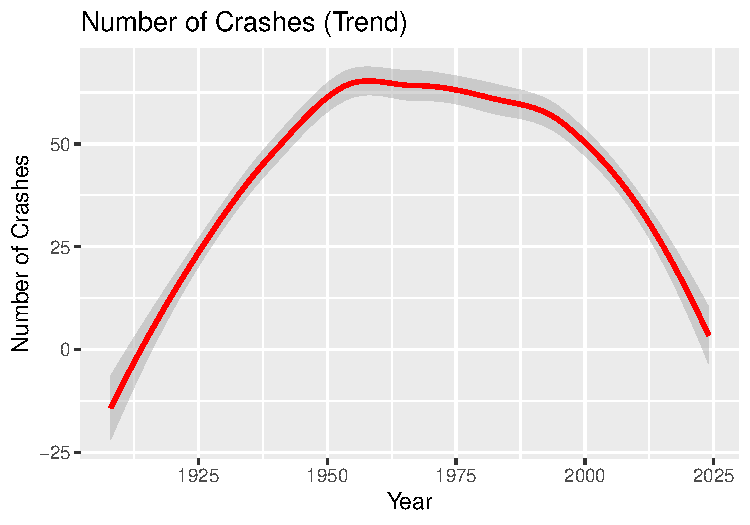
\includegraphics[width=\textwidth]{figures/crashes-trend.pdf}
  \end{subfigure}
  \caption{Number of crashes}
\end{figure}

\begin{figure}[htbp]
  \centering
  \begin{subfigure}[b]{0.48\textwidth}
    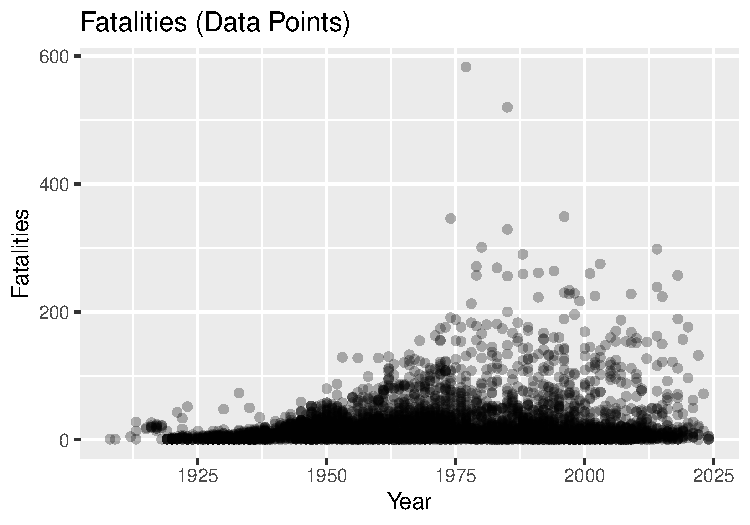
\includegraphics[width=\textwidth]{figures/fatalities-data.pdf}
  \end{subfigure}
  \hfill
  \begin{subfigure}[b]{0.48\textwidth}
    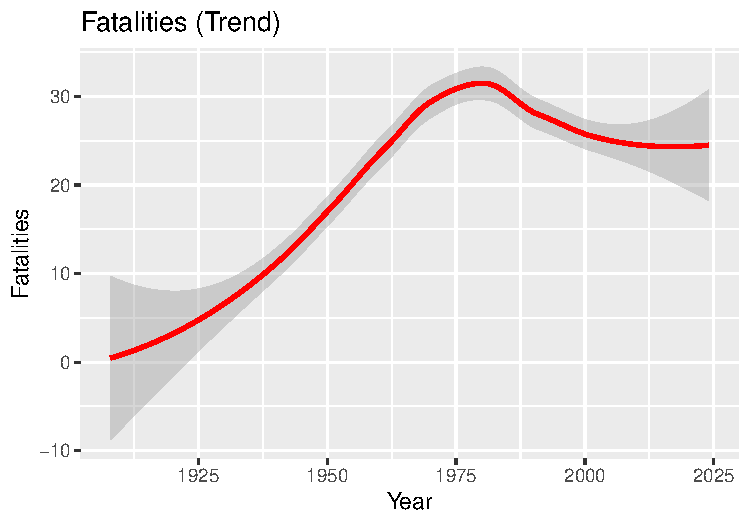
\includegraphics[width=\textwidth]{figures/fatalities-trend.pdf}
  \end{subfigure}
  \caption{Number of fatalities}
\end{figure}

\begin{figure}[htbp]
  \centering
  \begin{subfigure}[b]{0.48\textwidth}
    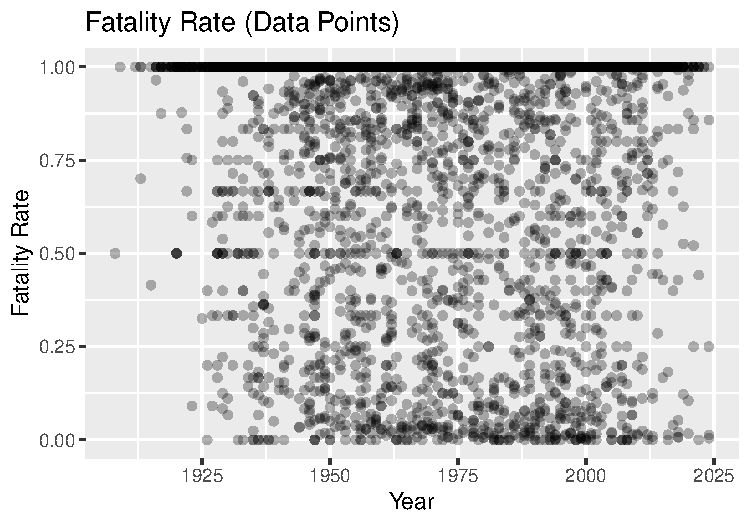
\includegraphics[width=\textwidth]{figures/fatality-rate-data.pdf}
  \end{subfigure}
  \hfill
  \begin{subfigure}[b]{0.48\textwidth}
    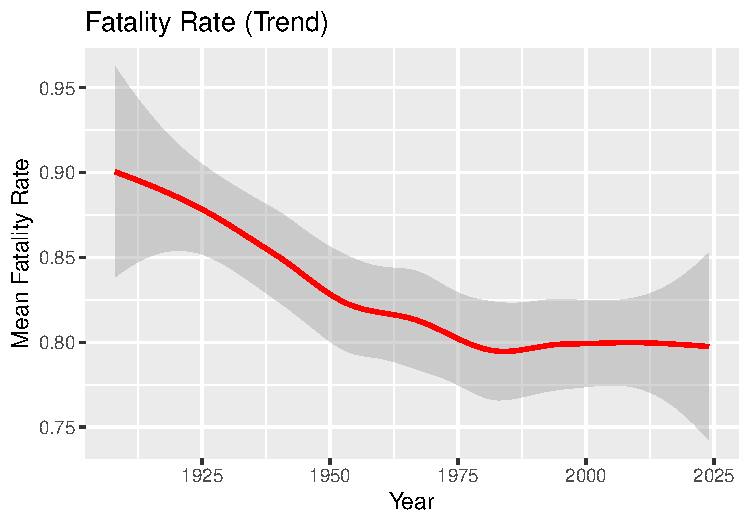
\includegraphics[width=\textwidth]{figures/fatality-rate-trend.pdf}
  \end{subfigure}
  \caption{Fatality rate}
\end{figure}

To conduct a modern analysis on plane crash fatalities, we do not want to include observations from far back in the history. We need some reasonable cutoff point that keeps sufficient amount of data and allows us to model modern aircraft data. The fatalities trend shows a turning point around 1975, so it is reasonable to choose that as our observation cutoff year. This filtering brings our total observation count from 5013 down to 2188, so we are still left with plenty of data. We also only include observations from manufacturers with at least 10 crashes present in the data to stabilize the no pooling and partial pooling models. This brought our data down to 1766 observations.

1975 is a good cutoff date, because it resembles a period that shares lots of characteristics with modern flight travel. The 1950s and 1960s saw an upsurge in commercial flights, aircraft carriers, and international flying routes \cite{airwaysmag_commercial_flight}. This upsurge was accompanied by great technological innovations. The most notable ones were the jet engine in the 1950s (safer and more reliable than the earlier piston engines) and the introduction electronic instruments to the cockpit in the 1970s. \cite{allianz_aviation_safety}

\begin{figure}[htbp]
  \centering
  \begin{subfigure}[b]{1.0\textwidth}
    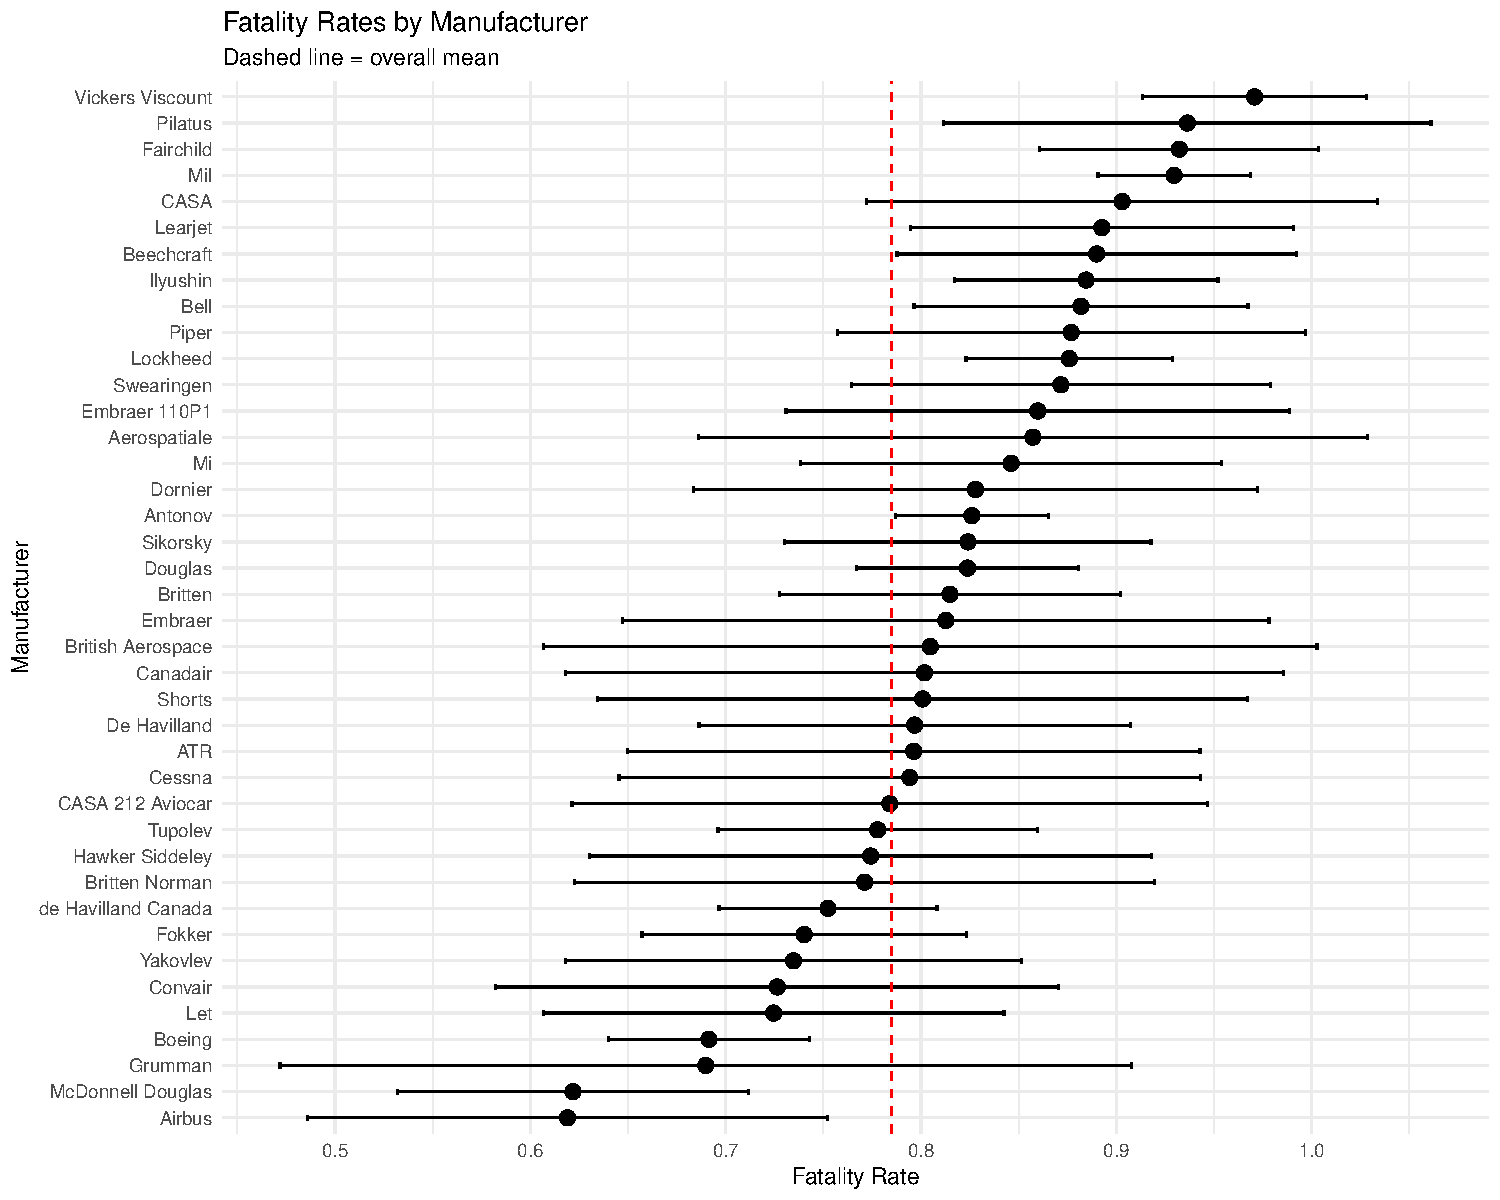
\includegraphics[width=\textwidth]{figures/fatality_rates-by-manuf.pdf}
  \end{subfigure}
  \caption{Fatality rates by manufacturer}
\end{figure}



\section{Literature Review}

% ARE THESE NECESSARY??
% \begin{figure}[htbp]
%   \centering
%   \begin{subfigure}[b]{0.48\textwidth}
%     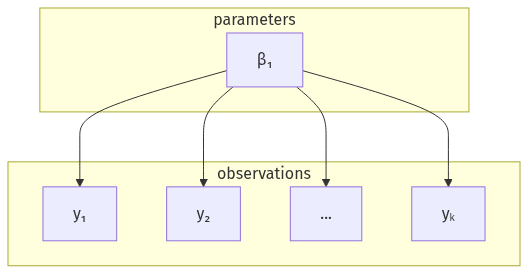
\includegraphics[width=\textwidth]{figures/non-hierarchical_model_complete_pooling.png}
%     \caption{complete pooling}
%   \end{subfigure}
%   \hfill
%   \begin{subfigure}[b]{0.48\textwidth}
%     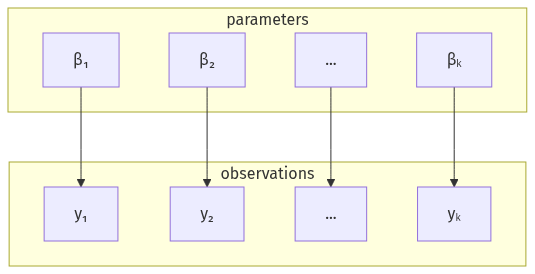
\includegraphics[width=\textwidth]{figures/non-hierarchical_model_no_pooling.png}
%     \caption{no pooling}
%   \end{subfigure}

%   \caption{Non-hierarchical models}
% \end{figure}

\subsection{Complete pooling (non-hierarchical)}

\begin{align*}
  fatalityRate_i & \sim \text{Normal}(\mu, \sigma) \\
  \mu            & \sim \text{Prior}               \\
  \sigma         & \sim \text{Prior}
\end{align*}

A complete pooling model assumes that all fatalities are sampled from a single model. In our plane crash example this would mean that we assume that all crashes follow the same distribution regardless of hierarchies like manufacturer or location.\\

\subsection{No pooling (non-hierarchical)}
\begin{align*}
  fatalityRate_{ij} & \sim \text{Normal}(\mu_j, \sigma) \\
  \mu_j             & \sim \text{Prior}                 \\
  \sigma            & \sim \text{Prior}
\end{align*}

A no pooling model model assumes that each entity in the hierarchy follows its own distribution. In our case, each manufacturer would have their own mean and this way, the differences between manufacturers is captured. The problem with this approach is overfitting. If a manufacturer has only few crashes, the model is fitted for the manufacturer with little to no data.

\subsection{Partial pooling (hierarchical)}

% NECESSARY??
% \begin{figure}[htbp]
%   \centering
%   \begin{subfigure}[b]{0.48\textwidth}
%     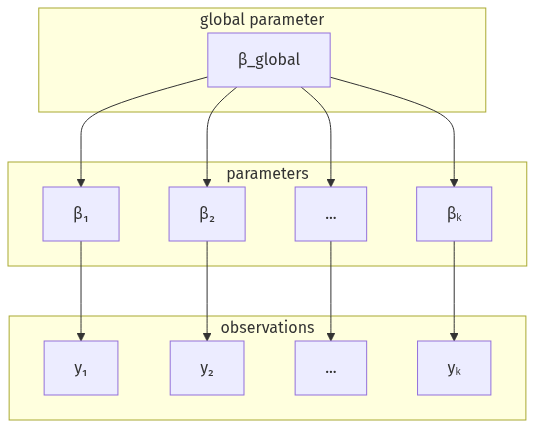
\includegraphics[width=\textwidth]{figures/hierarchical_model.png}
%     \caption{Partial pooling}
%   \end{subfigure}
%   \caption{hierarchical model}
% \end{figure}

\begin{align*}
  fatalityRate_{ij} & \sim \text{Normal}(\mu_j, \sigma)      \\
  \mu_j             & \sim \text{Normal}(\mu_{global}, \tau) \\
  \mu_{global}      & \sim \text{Prior}                      \\
  \tau              & \sim \text{Prior}                      \\
  \sigma            & \sim \text{Prior}
\end{align*}

Similar to the no pooling model, partial pooling also assumes that each manufacturer has their own distribution. Contrary to no pooling models, partial pooling models assume that the parameters for each manufacturer come from a global distribution. This solves the problem of overfitting caused by manufacturers with few data points. This problem is solved by borowing strength from the global distribution of parameters.


\section{Model descriptions}
For our modeling task, we used three different model types: a fully separate model with no pooling, a complete pooling model, and a partially pooled model. The non-hierarchical models (complete and no-pooling models) are used for baseline comparisons for the hierarchical model (partial pooling), which is expected to perform the best for this task. With these models, we are modeling the fatality rate for a given plane crash and using binomial likelihood.

We use the logit function to bound the outputs of our model between 0 and 1. The logit function is

\[
  \operatorname{logit}(p_i) = \ln\left(\frac{p_i}{1-p_i}\right)
\]

When $\eta_i$ is a linear predictor,

\begin{align*}
  \operatorname{logit}(p_i)                          & = \eta_i                                             \\
  \exp\left(\ln\left(\frac{p_i}{1-p_i}\right)\right) & = \exp(\eta_i)                                       \\
  \frac{p_i}{1-p_i}                                  & = \exp(\eta_i) \quad \quad || \text{solving for }p_i \\
  p_i                                                & = \frac{\exp(\eta_i)}{1 + \exp(\eta_i)}
\end{align*}

This way our linear predictors $\eta_i$ can produce outputs in $(-\infty, \infty)$ and the fatality rates $p_i$ stay in [0,1].

\subsection{Complete pooling (non-hierarchical model)}

\begin{lstlisting}
complete_pool_formula <- bf(
    fatalities | trials(aboard) ~ 1 + year_scaled,
    family = binomial(link = "logit")
)

priors <- c(
    prior(normal(1.4, 1), class = Intercept),
    prior(normal(0, 0.5), class = b)
)

complete_pool_model <- brm(
    formula = complete_pool_formula,
    prior = priors,
    data = crashes,
    seed = 42,
    refresh = 0,
    cores = 4
)
\end{lstlisting}

With $i$ reprecenting individual crashes, $n_i$ reprecenting the amount of people aboard on the crash and $p_i$ reprecenting the fatality probability of a crash, the model can be written as:

\begin{align*}
  \text{Likelihood:} \quad &                                       \\
  y_i                      & \sim \text{Binomial}(n_i, p_i)        \\
  \text{logit}(p_i)        & = \alpha + \beta \cdot year\_scaled_i \\[1em]
  \text{Priors:} \quad     &                                       \\
  \alpha                   & \sim \mathcal{N}(1.4, 1)              \\
  \beta                    & \sim \mathcal{N}(0, 0.5)
\end{align*}

The complete pooling model is the simplest of our three models. The model assumes that each manufacturer shares the same intercept and linear coefficient. The weakness of this model is that it is not able to capture the potential differences between the manufacturers.


\subsection{No pooling (non-hierarchical model)}

\begin{lstlisting}

no_pool_formula <- bf(
    fatalities | trials(aboard) ~ 0 + aircraft_manufacturer + aircraft_manufacturer:year_scaled,
    family = binomial(link = "logit")
)

priors <- c(
    prior(normal(0, 1), class = b)
)

no_pool_model <- brm(
    formula = no_pool_formula,
    prior = priors,
    data = crashes,
    seed = 42,
    refresh = 0,
    cores = 4
)
\end{lstlisting}

This model treats every airplane manufacturer as their own independent entity, without sharing any information across any other possible grouping in the data. With $i$ being the index of a plane crash and $m[i]$ being the manufacturer $m$ for crash $i$, we can write the model as:

\begin{align*}
  \text{Likelihood:} \quad &                                                           \\
  y_i                      & \sim \text{Binomial}(n_i, p_i)                            \\
  \text{logit}(p_i)        & = \alpha_{m[i]} + \beta_{m[i]} \cdot year\_scaled_i       \\[1em]
  \text{Priors:} \quad     &                                                           \\
  \alpha_m                 & \sim \mathcal{N}(0, 1) \quad \text{for } m = 1, \ldots, M \\
  \beta_m                  & \sim \mathcal{N}(0, 1) \quad \text{for } m = 1, \ldots, M
\end{align*}

This means that the model assumes that each crash has its own fatality rate based on the manufacturer and the year, and crashes from other manufacturers do not influence each other in any way. With this model, the estimates for manufacturers with only a few crashes in the data become unstable, because they can't borrow information from other manufacturers.

\subsection{Partial pooling (hierarchical model)}

\begin{lstlisting}
hierarchical_formula <- bf(
  fatalities | trials(aboard) ~ 1 + year_scaled + (1 + year_scaled | aircraft_manufacturer),
  family = binomial(link = "logit")
  )

priors <- c(
    prior(normal(1.4, 1), class = Intercept),
    prior(normal(0, 0.5), class = b),
    prior(normal(0, 0.6), class = sd),
    prior(lkj(2), class = cor)
  )

partial_pool_model <- brm(
  formula = hierarchical_formula,
  prior = priors,
  data = crashes,
  seed = 42,
  control = list(adapt_delta = 0.95),
  refresh = 0,
  cores = 4
)
\end{lstlisting}

\begin{align*}
  \text{Likelihood:} \quad     &                                                                                                           \\
  y_i                          & \sim \text{Binomial}(n_i, p_i)                                                                            \\
  \text{logit}(p_i)            & = \alpha_0 + \beta_0 \cdot year\_scaled_i + \alpha_{m[i]} + \beta_{m[i]} \cdot year\_scaled_i             \\[1em]
  \text{Random effects:} \quad &                                                                                                           \\
  \begin{bmatrix}
    \alpha_m \\
    \beta_m
  \end{bmatrix}             & \sim \mathcal{N}\left(
  \begin{bmatrix}
    0 \\
    0
  \end{bmatrix}, \boldsymbol{\Sigma}\right), \quad \boldsymbol{\Sigma} = \begin{bmatrix}
                                                                           \sigma_\alpha^2                 & \rho \sigma_\alpha \sigma_\beta \\
                                                                           \rho \sigma_\alpha \sigma_\beta & \sigma_\beta^2
                                                                         \end{bmatrix} \\[1em]
  \text{Priors:} \quad         &                                                                                                           \\
  \alpha_0                     & \sim \mathcal{N}(1.4, 1)                                                                                  \\
  \beta_0                      & \sim \mathcal{N}(0, 0.5)                                                                                  \\
  \sigma_\alpha, \sigma_\beta  & \sim \mathcal{N}^+(0, 0.6)                                                                                \\
  \rho                         & \sim \text{LKJ}(2)
\end{align*}

For the partially pooled model, we are predicting both a population level intercept and coefficient ($\alpha_0$ and $\beta_0$) and manufacturer level intercepts and coefficients ($\alpha_{m[i]}$ and $\beta_{m[i]}$). The partially pooled model is a combination of the techniques used in the no pooling model and the complete pooling model. The no pooling method assumed that each manufacturer had their own intercept and coefficient and the complete pooling model assumed that all manufacturers have the same intercept and coefficient. The partial pooling assumes that both of these conditions hold.


\subsection{Prior selection}
\subsubsection*{Global intercept}
For the global intercept term $\alpha$, we can use a weakly informative prior by using the observed fatality rate of $\approx 0.8$ from the data. We can use a normal distribution with the mean value coming from the observed fatality rate transformed onto the logit scale by

$$\operatorname{logit}(p) = \ln\!\left(\frac{p}{1-p}\right).$$

For example, $\operatorname{logit}(0.8) \approx 1.386$, which we round to $1.4$. For a weakly informative prior like ours, a standard deviation of $1$ is a reasonable choice to keep the coefficient in a reasonable ballpark without adding too much constraint.

\subsubsection*{Global year coefficient}
For the global $\beta$ coefficient on the normalized year, we can be more conservative. The fatality rate plot shows only little yearly change, so it is reasonable to constrain the $\beta$ prior to smaller values. A normal distribution with mean $0$ and standard deviation $0.5$ seems reasonable. The 95\% credible interval for $\beta$ is then approximately $[-1.0, 1.0]$. This is also a weakly informative prior.

\subsubsection*{Manufacturer level priors}
For the manufacturer level intercept terms \(\alpha_m\) and \(\beta_m\) in the fully separate model, we should use the same weakly informative priors that we use for the global terms. However, to achieve this, brms wants a separate prior set for every manufacturer, which makes the task incredibly cumbersome. Thus, we use a weakly informative prior of a normal distribution with a mean of 0 and a standard deviation of 1, which is a safe choice and should still result in a good model.

\subsubsection*{Group level standard deviation}
In our hierarchical model, we have an extra intercept term based on the aircraft manufacturer, which is drawn from a halfnormal distribution with most mass around 0 and a standard deviation of $\sigma$. We need an appropriate prior for this group level standard deviation term $\sigma$. Observing the manufacturer level data, we see that the fatality rates fall roughly between 0.6 and 0.95 across all manufacturers. We can assume that this interval corresponds to $\pm2\sigma$, so it covers 95\% of the groups. Converting this to the logit scale, we can calculate

$$\sigma: 2\sigma \approx \frac{\operatorname{logit}(0.95) - \operatorname{logit}(0.6)}{2} \Rightarrow \sigma = \frac{\operatorname{logit}(0.95) - \operatorname{logit}(0.6)}{4} \approx 0.635$$.

A weakly informative halfnormal distribution with a standard deviation of 0.6 should be a good prior choice. The mean of this distribution is $E[X] = \sigma\sqrt{\frac{2}{\pi}} \approx 0.479$, which seems reasonable for our model.

\subsubsection*{Correlation coefficient $\rho$}

For the correlation coefficient $\rho$ we use an LKJ distribution. The distribution is designed for correlation matricies. The shape parameter $\eta$ in $\operatorname{LKJ}(\eta)$ is 2 in our model. When $\eta>1$, the prior causes the model to be skeptical of strong correlations. In more technical terms, the distribution is a bell shaped distribution centered at zero.


\section{Model fitting}
\subsection{No pooling model}

\subsubsection*{Convergence diagnostics}
The \(\hat{R}\) value for each of the parameters is 1.00, which means all coefficients converged properly. The bulk ESS values vary on the scale [4200, 5800] and the tail ESS values on the scale [2600, 3500]. These ESS values are far more than is needed for a reliable posterior estimation, so no problems there. The model had no divergences.

\subsubsection*{Posterior predictive check}
The posterior predictive checks compare the real observed fatalities with the ones generated from our fitted model. If the model is good, the simulated figures should resemble the real figures.

\begin{figure}[htbp]
  \centering
  \begin{subfigure}[b]{0.48\textwidth}
    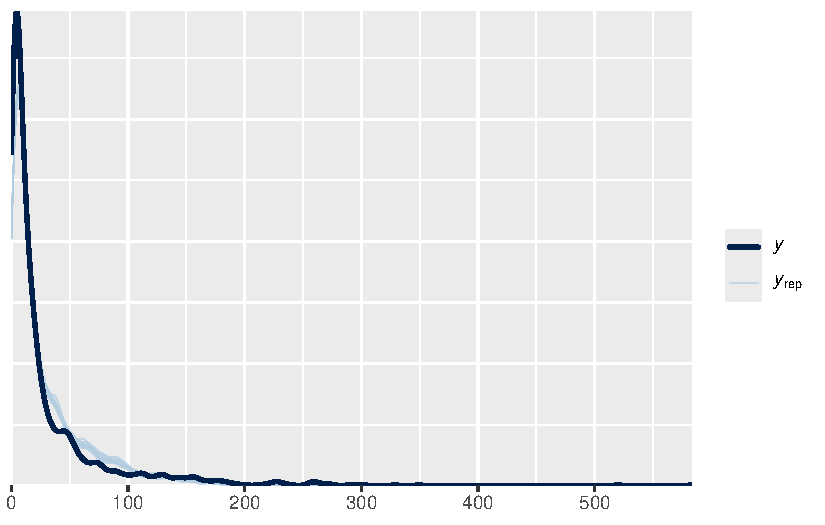
\includegraphics[width=\textwidth]{figures/no_pool_ppcheck.pdf}
    \caption{No pool -model ECDF}
  \end{subfigure}
  \hfill
  \begin{subfigure}[b]{0.48\textwidth}
    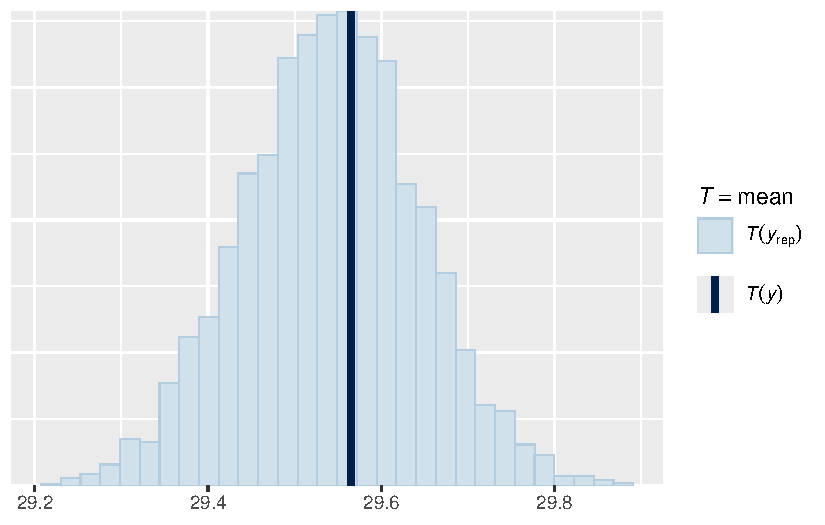
\includegraphics[width=\textwidth]{figures/no_pool_ppcheck_mean.pdf}
    \caption{No pool -model mean comparison}
  \end{subfigure}
  \hfill
  \begin{subfigure}[b]{0.48\textwidth}
    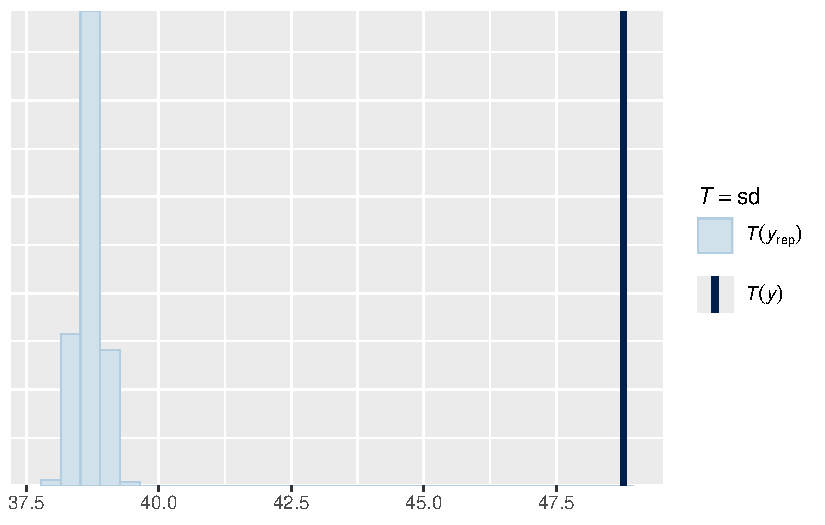
\includegraphics[width=\textwidth]{figures/no_pool_ppcheck_sd.pdf}
    \caption{No pool -model sd comparison}
  \end{subfigure}

  \caption{No pool -models ppcheck plots}
\end{figure}

The ECDF (empirical cumulative distribution function) shows that the model is slightly off when compared to the real data. We can see that at the start, the observed ECDF rises faster and higher than the model ECDF, indicating that model predicts less crashes with close to 0 fatalities. However, in the 25-100 fatalities area, the observed ECDF lags behind the model ECDF meaning that the model estimates more crashes that lead to those fatality numbers.

The mean comparison plot shows that the true fatalities mean lies close to the center of the model simulated fatalities distribution, meaning that the model estimates the overall mean fatality rate correctly.

The standard deviation comparison plot shows that the true fatalities standard deviation is much larger than what the model estimates. In other words, the model predicts too little variability and is under-dispersed.

\subsubsection*{Prior sensitivity analysis}

We conduct a prior sensitivity analysis on this model by trying out 3 different priors and comparing the estimated parameters of 4 manufacturers. The priors we are using are:
\begin{itemize}
  \item \textbf{Model prior:} Normal(0, 1) (same as the model).

  \item \textbf{Wide prior:} Normal(0, 3) (a much wider distribution).

  \item \textbf{Shifted prior:} Normal(2, 1) (shifted to the right).
\end{itemize}

\begin{table}[h]
  \centering
  \begin{tabular}{llcc}
    \hline
    \textbf{Prior Distribution} & \textbf{Manufacturer} & \textbf{$\alpha$} & \textbf{$\beta$} \\
    \hline
    \multirow{4}{*}{Model Normal(0, 1)}
                                & Boeing                & 0.72              & $-0.34$          \\
                                & Bell                  & 1.94              & 0.82             \\
                                & Lockheed              & 0.16              & 1.00             \\
                                & Mil                   & 4.34              & $-1.67$          \\
    \hline
    \multirow{4}{*}{Wide Normal(0, 3)}
                                & Boeing                & 0.72              & $-0.34$          \\
                                & Bell                  & 2.20              & 0.63             \\
                                & Lockheed              & 0.16              & 1.00             \\
                                & Mil                   & 5.16              & $-2.30$          \\
    \hline
    \multirow{4}{*}{Shifted Normal(2, 1)}
                                & Boeing                & 0.72              & $-0.34$          \\
                                & Bell                  & 1.96              & 0.96             \\
                                & Lockheed              & 0.16              & 1.00             \\
                                & Mil                   & 4.40              & $-1.70$          \\
    \hline
  \end{tabular}
  \caption{Parameter estimates for manufacturers under different prior distributions.}
  \label{tab:helicopter_params}
\end{table}

We can see that the parameters do not vary much. For manufacturers with many observations in the data (Boeing: 248 observations, Lockheed: 106 observations), the parameters are identical for every prior. For manufacturers with a fewer number of observations (Mill: 41 observations, Bell: 33 observations), the parameter values show more variance.
$$\text{Mill:}$$
$$\operatorname{Var}(\alpha ) \approx 0.21, \operatorname{Var}(\beta) \approx 0.11$$
$$\text{Bell:}$$
$$\operatorname{Var}(\alpha ) \approx 0.02, \operatorname{Var}(\beta) \approx 0.03$$
These variances are tolerable and still show the same trend, just in different strengths.
The results show that the model is stable under reasonable prior changes, and the main conclusions drawn from the model do not depend on the chosen prior.


\subsection{Complete pooled model}

\subsubsection*{Convergence diagnostics}
The \(\hat{R}\) value for both the intercept term and the year coefficient is 1.00, indicating almost perfect chain overlapping. For both parameters, the bulk ESS values are over 3000 and the tail ESS values are over 2000. These values are great and definitely sufficient. The model had no divergences.

\subsubsection*{Posterior predictive check}
\begin{figure}[htbp]
  \centering
  \begin{subfigure}[b]{0.48\textwidth}
    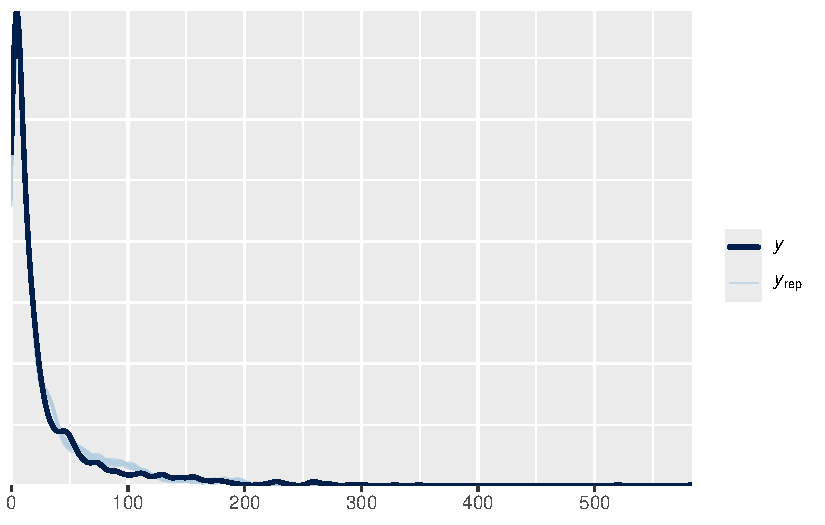
\includegraphics[width=\textwidth]{figures/complete_pool_ppcheck.pdf}
    \caption{Complete pool -model ECDF}
  \end{subfigure}
  \hfill
  \begin{subfigure}[b]{0.48\textwidth}
    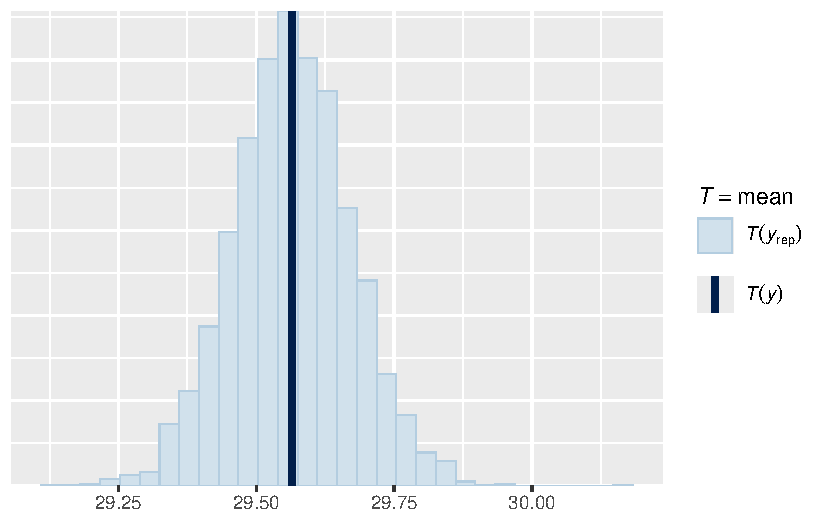
\includegraphics[width=\textwidth]{figures/complete_pool_ppcheck_mean.pdf}
    \caption{Complete pool -model mean comparison}
  \end{subfigure}
  \hfill
  \begin{subfigure}[b]{0.48\textwidth}
    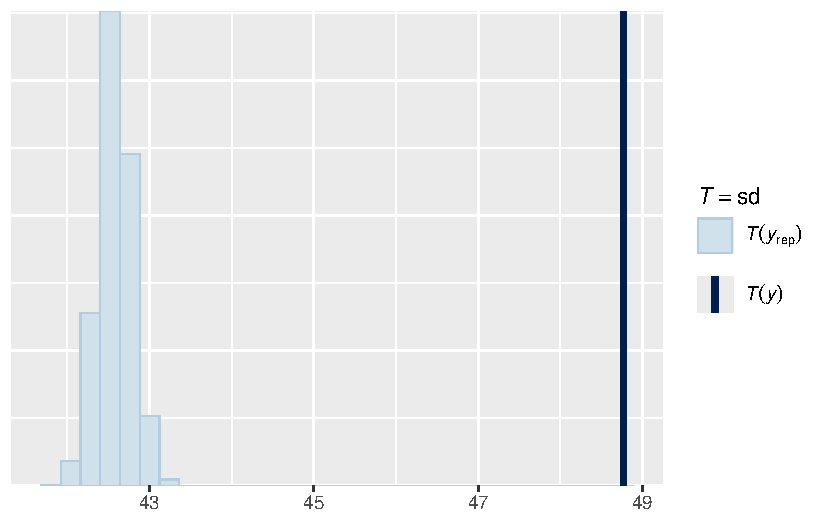
\includegraphics[width=\textwidth]{figures/complete_pool_ppcheck_sd.pdf}
    \caption{Complete pool -model sd comparison}
  \end{subfigure}

  \caption{Complete pool -models ppcheck plots}
\end{figure}

The complete pooling model ECDF follows the observed ECDF better at low fatalities than the no pooling model, but it still struggles in the 25-100 fatalities region.

The mean comparison plot shows that the observed mean is almost at the exact center of the model simulated fatalities distribution, meaning that this model also estimates the overall fatality rate correctly.

The standard deviation comparison plot shows that this model is also under-dispersed, but the effect is smaller than with the no pooling model.


\subsubsection*{Prior sensitivity analysis}

We conduct a prior sensitivity analysis on this model by trying out 3 different prior settings and comparing the estimated parameters. The priors we are using are:
\begin{itemize}
  \item \textbf{Model prior:} Intercept prior: Normal(1.4, 1), year coefficient prior: Normal(0, 0.5) (same as the model).

  \item \textbf{Wide prior:} Intercept prior: Normal(1.4, 3), year coefficient prior: Normal(0, 1.5) (3 times as wide for both).

  \item \textbf{Shifted prior:} Intercept prior: Normal(3.4, 1), year coefficient prior: Normal(2, 0.5) (both priors shifted by 2 to the right).
\end{itemize}

\begin{table}[h]
  \centering
  \begin{tabular}{lcc}
    \hline
    \textbf{Prior Distribution} & \textbf{$\alpha$} & \textbf{$\beta$} \\
    \hline
    Model prior                 & 0.81              & $-0.18$          \\
    Wide prior                  & 0.81              & $-0.18$          \\
    Shifted prior               & 0.81              & $-0.18$          \\
    \hline
  \end{tabular}
  \caption{Parameter estimates under different prior distributions.}
  \label{tab:model_comparison}
\end{table}

The parameters are identical for all three priors. From these results it can be concluded that the model is very insensitive to the prior choice.

\subsection{Partial pooling model}

\subsubsection*{Convergence diagnostics}

\begin{table}[htbp]
  \centering
  \caption{Convergence Diagnostics for Partial Pooling Model}
  \begin{tabular}{lccc}
    \hline
    Parameter                        & $\hat{R}$ & Bulk ESS & Tail ESS \\
    \hline
    \multicolumn{4}{l}{\textit{Multilevel Hyperparameters}}            \\
    $\sigma_\alpha$ (SD Intercept)   & 1.00      & 875      & 1707     \\
    $\sigma_\beta$ (SD year\_scaled) & 1.01      & 779      & 1184     \\
    $\rho$ (Correlation)             & 1.00      & 961      & 1537     \\
    \multicolumn{4}{l}{\textit{Fixed Effects}}                         \\
    $\alpha_0$ (Intercept)           & 1.01      & 511      & 959      \\
    $\beta_0$ (year\_scaled)         & 1.00      & 516      & 951      \\
    \hline
  \end{tabular}
  \label{tab:convergence}
\end{table}

The partial pooling model MCMC converged well with all $\hat{R}$ values smaller or equal to 1.01. Even though our process converged, the low ESS values are troublesome. Both bulk ESS and tail ESS values should be over 1000 in an ideal case. The models ESS values are relatively close to 1000 for the standard deviation and correlation parameters, but are far away from ideal for the intercept $\alpha_0$ and the coefficient $\beta_0$. We tried doubling the warmup and iteration counts to 1000 and 4000 respectively, but the ESS numbers stay the same. This means that especially for $\alpha_0$ and $\beta_0$, we don't have enough independent samples for truly reliable posterior estimates.

\subsubsection*{Posterior predictive check}

\begin{figure}[htbp]
  \centering
  \begin{subfigure}[b]{0.48\textwidth}
    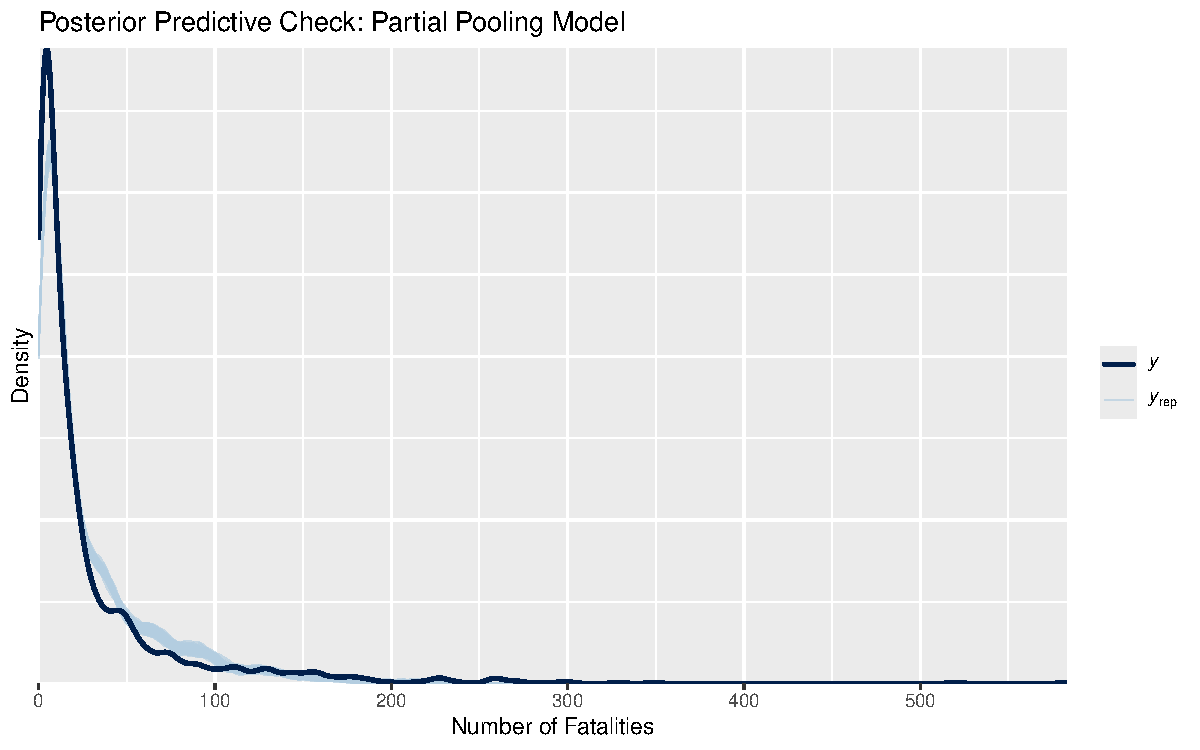
\includegraphics[width=\textwidth]{figures/partial_pool_ppcheck.pdf}
    \caption{Partial pool -model ECDF}
  \end{subfigure}
  \hfill
  \begin{subfigure}[b]{0.48\textwidth}
    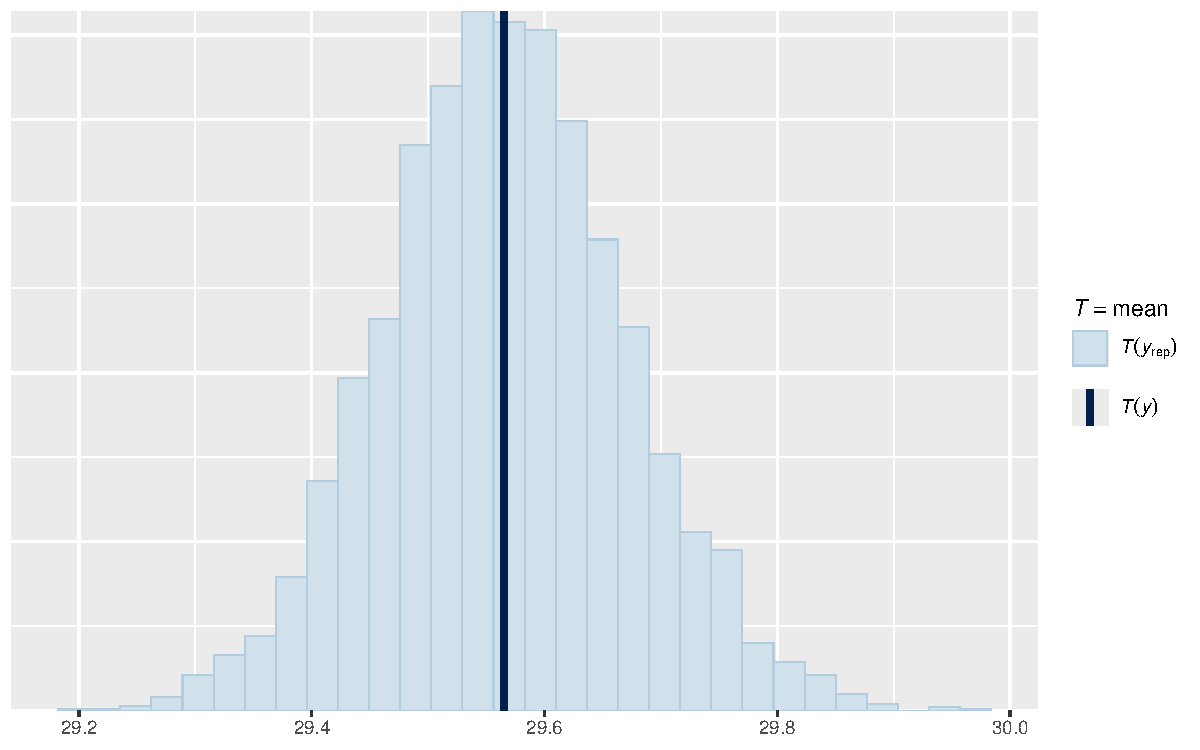
\includegraphics[width=\textwidth]{figures/partial_pool_ppcheck_mean.pdf}
    \caption{Partial pool -model mean comparison}
  \end{subfigure}
  \hfill
  \begin{subfigure}[b]{0.48\textwidth}
    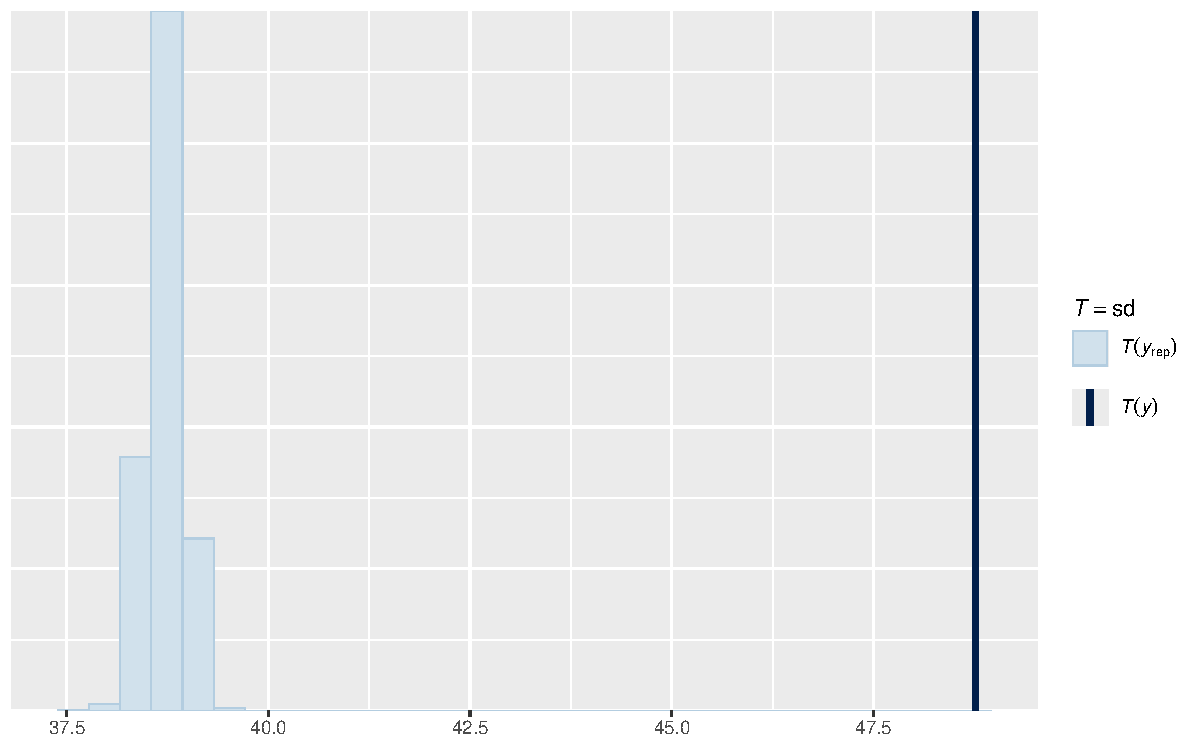
\includegraphics[width=\textwidth]{figures/partial_pool_ppcheck_sd.pdf}
    \caption{Partial pool -model sd comparison}
  \end{subfigure}

  \caption{Partial pool -models ppcheck plots}
\end{figure}

The ECDF of of the partially pooled model matches the original observations fairly well. Same for observed mean in the (b) graph. The standard deviation comparison has the same problem as the other two models that it is under-dispersed.

\subsubsection*{Prior sensitivity analysis}

For the partial pooling model, we'll analyse how changing our prior assumtions on how similar manufacturers are, affects the posterior predictions. We will do this by using three differnt priors four our standard deviations $\sigma$:

\begin{itemize}
  \item \textbf{Baseline}: $\sigma \sim \mathcal{N}(0, 0.6)$ -- (original)
  \item \textbf{Tight}: $\sigma \sim  \mathcal{N}(0, 0.3)$ -- (assumes manufacturers more similar)
  \item \textbf{Wide}: $\sigma \sim \mathcal{N}(0, 1.2)$ -- (assumes manufacturers differ more)
\end{itemize}

\begin{table}[h]
  \centering
  \caption{Comparison of posterior means with different priors}
  \label{tab:posterior_comparison}
  \begin{tabular}{lccc}
    \hline
    Prior Scenario & Intercept Mean & Year Effect Mean & SD Manufacturer Mean \\
    \hline
    Baseline       & 1.271          & 0.019            & 1.205                \\
    Tight          & 1.263          & 0.024            & 1.037                \\
    Wide           & 1.280          & 0.016            & 1.295                \\
    \hline
  \end{tabular}
\end{table}

The means don't show notisable effects from different prior choises. The standard deviation is affected by changing the prior distributions for it, but this is fine. The standard deviation priors should only affect the standard deviation posteriors. Thus we can conclude that our model is robust.



\section{Model comparison}

To compare the three models, we use LOO-CV (Leave-One-Out Cross-Validation), that has the basic idea of 1) Remove an observation \(i\), 2) Train the model, 3) Predict the observation \(i\). Then measure how well the model performed and compare the models. We measure the ELPD (Expected Log Predictive Density) and SE (Standard Error) for all models and then compare them with each other. We use the partial pooling model as the baseline to compare other models to.

\begin{table}[h]
  \centering
  \begin{tabular}{lrrr}
    \hline
    Model                 & elpd\_diff & se\_diff & $\left|\frac{\text{elpd\_diff}}{\text{se\_diff}}\right|$ \\
    \hline
    partial\_pool\_model  & 0.0        & 0.0      & --                                                       \\
    no\_pool\_model       & -16.5      & 13.3     & 1.2406                                                   \\
    complete\_pool\_model & -1944.8    & 692.3    & 2.8103                                                   \\
    \hline
  \end{tabular}
  \caption{LOO-CV model comparison results}
  \label{tab:model_comparison_ratio}
\end{table}


A good rule of thumb is that if \(\text{elpd-diff} < 1 \cdot \text{se-diff}\), the models are close to equal and if \(\text{elpd-diff} > 2 \cdot \text{se-diff}\), there is a clear difference between the models. A higher ELPD value indicates better performance. Taking this into consideration, we can analyze the results.

The no pooling model seems to perform slightly worse than the partial pooling model, but the ratio of 1.24 is still close to 1 and could just be due to random noise, so no clear conclusions can be drawn from this.

The complete pooling model, however, can be reported to perform significantly worse than the other two models. The reason for this is most likely that the model fails to capture the manufacturer level differences, and therefore predicts incorrectly for most crashes.


\section{Problems and potential improvements}

Although the partial pooling model performs best according to LOO cross-validation, none of the three models succeeds in accurately modeling the structure of the real data, revealed by the predictive posterior check analysis.

The two non-hierarchical models have their obvious limitations, but the interesting question is: Why does the hierarchical model fail? On paper, it should perform well, because it uses population level information as well as captures the manufacturer level differences. Evidently, it still has its limitations.

The problem with all of our models seemed to be, that they were under-dispersed, meaning that the underestimated the variance. The reason for this mainly comes from our use of binomial likelihood for predicting the fatalities. The variance formula of binomial likelihood for an observation \(i\) is
$$\operatorname{Var}(Y_i) = n_i p_i (1 - p_i).$$
This formula is fixed once \(n_i\) and \(p_i\) are known and is bounded by \(n_i / 4\) (when \(p_i = 0.5\)). The true variances in the observed data were shown to be much larger than the models', because the binomial variance simply cannot reach the true variability values. As a potential improvement for the models, a different likelihood function, that could combat this under-dispersion problem, should be used.

Another reason, that our models fail is much simpler. Airplane crashes simply cannot be modeled accurately, especially with so little information. There are countless factors that can affect the fatality rate of a crash and a there is a lot of randomness included. One could try to add more predictors and see if it yields better results. But even with more predictors included, the results would still most likely be inaccurate, but perhaps better than what we reached.



\section{Conclusion}

In our report, we modeled fatality rate trends with hierarchical and non-hiearchical models. We used three types of models: complete pooling, no pooling and partial pooling models. From these models the partial pooling model performed the best with the no pooling model coming in a close second. We used LOO-CV to compare our models.

One of our research questions was are there differences in the fatality rates of manufacturers. The fact that the partial pooling and no pooling models performed well would suggest that fatalities are modeled better assuming that each manufacturer has their own parameters and distributions.

According to our prior sensitivity analysis, the models were quite unaffected from changes in priors. This means that our models are able to model the fatality rates well without the priors having a too big of an affect on the model.

In our posterior predictive analysis, we noticed that our models weren't capturing the variance of the original observations. The variance of our models was too small. This was due to the fixed maximum variance of the binomial model being too small to correctly model the real crash variance.

\section{What we learned}

The project was a great summary of the key consepts taught on the Bayesian Data Analysis course. During the course we aquired basic skills in bayesian data analysis and during the project we got to use them in practise and deepen our understanding about the methods.

In this report we discussed things like hierarchical and non-hierarchical models, how to choose priors and test the effects of these priors on the predictions, how to run MCMC simulations and how to compare and evaluate the models these simulations suggest.

Running MCMC simulations is computationally expensive and the project showed the importance of access to cloud computing resources. Running the MCMC code could take over 30 minutes on old hardware while it took 5--10 minutes to run on modern cloud hardware in JupyterHub.


\printbibliography

\end{document}